\newcommand{\downloaderTagResultsAucTable}{
    \begin{table}[H]
        \centering
        \begin{tabular}{|p{2,8cm}||p{2,8cm} p{2,8cm} p{2,8cm}|}
            \hline
            Downloader Tag & ALOHA & Joint Embedding & Proposed Model \\
            \hline
            AUC-ROC & \textBF{0.535$\pm$0.036} & 0.499$\pm$0.022 & 0.510$\pm$0.020 \\
            \hline
        \end{tabular}
        \caption{AUC-ROC (Area Under Curve) of the different models for the \textbf{Downloader Tag} prediction task. Results were aggregated over \textBF{3} training runs with different weight initializations and minibatch orderings. Best results are shown in \textbf{bold}.} \label{tab:downloaderTag_auc}
    \end{table}
}

\newcommand{\downloaderTagResultsAtFprTable}{
    \begin{center}
        \begin{longtable}[c]{|p{3,2cm}||p{1,8cm} p{1,8cm} p{1,8cm} p{1,8cm} p{1,8cm}|}
            \hline
            Downloader Tag & \multicolumn{5}{c|}{{FPR}} \\
            & $10^{-5}$ & $10^{-4}$ & $10^{-3}$ & $10^{-2}$ & $10^{-1}$ \\
            \hline
            \endfirsthead

            \caption*{\raggedright ...continued from previous page} \\
            \hline
            Downloader Tag & \multicolumn{5}{c|}{\textbf{FPR}} \\
            & $10^{-5}$ & $10^{-4}$ & $10^{-3}$ & $10^{-2}$ & $10^{-1}$ \\
            \hline
            \endhead

            \caption*{\raggedleft ...continued on next page} \\
            \endfoot

            \caption{Mean and standard deviation results (TPR, Accuracy, Recall, Precision and F1-Score) of the different models for the \textbf{Downloader Tag} prediction task at different \textbf{FPR}s (\textit{False Positive Rates}). Results were aggregated over \textBF{3} training runs with different weight initializations and minibatch orderings. Best results are shown in \textbf{bold}. Under \textbf{TPR} results are also presented the percentage reduction in mean detection error and in ROC curve standard deviation introduced by the \textit{Proposed Model} with respect to both \textit{ALOHA} model and \textit{Joint Embedding}.} \label{tab:downloaderTag_results_at_fpr} \\
            \endlastfoot

            \multicolumn{6}{|c|}{\textbf{TPR}} \\
            \hline
            ALOHA & 0.000$\pm$0.000 & 0.000$\pm$0.000 & 0.000$\pm$0.000 & 0.010$\pm$0.003 & \textBF{0.132$\pm$0.019} \\
            Joint Embedding & 0.000$\pm$0.000 & 0.000$\pm$0.000 & 0.000$\pm$0.000 & \textBF{0.012$\pm$0.005} & 0.100$\pm$0.027 \\
            Proposed Model & \textBF{0.002$\pm$0.003} & \textBF{0.002$\pm$0.003} & \textBF{0.004$\pm$0.003} & \textBF{0.012$\pm$0.005} & 0.118$\pm$0.029 \\
            \hline
            Error Reduction wrt \newline ALOHA & 0.2\% & 0.2\% & 0.4\% & 0.2\% & -1.6\% \\
            Error Reduction wrt \newline Joint Embedding & 0.2\% & 0.2\% & 0.4\% & 0.0\% & 2.0\% \\
            \hline
            Std Reduction wrt \newline ALOHA & 0.0\% & 0.0\% & 0.0\% & -66.7\% & -52.6\% \\
            Std Reduction wrt \newline Joint Embedding & 0.0\% & 0.0\% & 0.0\% & 0.0\% & -7.4\% \\
            \hline
            \multicolumn{6}{|c|}{\textbf{Accuracy}} \\
            \hline
            ALOHA & \textBF{0.933$\pm$0.000} & \textBF{0.933$\pm$0.000} & 0.932$\pm$0.000 & 0.926$\pm$0.000 & \textBF{0.849$\pm$0.002} \\
            Joint Embedding & \textBF{0.933$\pm$0.000} & \textBF{0.933$\pm$0.000} & \textBF{0.933$\pm$0.000} & 0.925$\pm$0.001 & 0.846$\pm$0.001 \\
            Proposed Model & \textBF{0.933$\pm$0.000} & \textBF{0.933$\pm$0.000} & \textBF{0.933$\pm$0.000} & \textBF{0.928$\pm$0.003} & 0.848$\pm$0.002 \\
            \hline
            \multicolumn{6}{|c|}{\textbf{Recall}} \\
            \hline
            ALOHA & 0.000$\pm$0.000 & 0.000$\pm$0.000 & 0.000$\pm$0.000 & 0.010$\pm$0.003 & \textBF{0.132$\pm$0.019} \\
            Joint Embedding & 0.000$\pm$0.000 & 0.000$\pm$0.000 & 0.000$\pm$0.000 & \textBF{0.012$\pm$0.005} & 0.100$\pm$0.027 \\
            Proposed Model & \textBF{0.002$\pm$0.003} & \textBF{0.002$\pm$0.003} & \textBF{0.004$\pm$0.003} & \textBF{0.012$\pm$0.005} & 0.118$\pm$0.029 \\
            \hline
            \multicolumn{6}{|c|}{\textbf{Precision}} \\
            \hline
            ALOHA & \textBF{1.000$\pm$0.000} & \textBF{1.000$\pm$0.000} & 0.000$\pm$0.000 & 0.077$\pm$0.017 & \textBF{0.087$\pm$0.012} \\
            Joint Embedding & \textBF{1.000$\pm$0.000} & \textBF{1.000$\pm$0.000} & 0.000$\pm$0.000 & 0.083$\pm$0.032 & 0.066$\pm$0.017 \\
            Proposed Model & \textBF{1.000$\pm$0.000} & \textBF{1.000$\pm$0.000} & \textBF{0.250$\pm$0.204} & \textBF{0.131$\pm$0.026} & 0.078$\pm$0.017 \\
            \hline
            \multicolumn{6}{|c|}{\textbf{F1 Score}} \\
            \hline
            ALOHA & 0.000$\pm$0.000 & 0.000$\pm$0.000 & 0.000$\pm$0.000 & 0.018$\pm$0.005 & \textBF{0.105$\pm$0.014} \\
            Joint Embedding & 0.000$\pm$0.000 & 0.000$\pm$0.000 & 0.000$\pm$0.000 & 0.021$\pm$0.009 & 0.080$\pm$0.021 \\
            Proposed Model & \textBF{0.004$\pm$0.006} & \textBF{0.004$\pm$0.006} & \textBF{0.008$\pm$0.006} & \textBF{0.022$\pm$0.008} & 0.094$\pm$0.022 \\
            \hline
        \end{longtable}
    \end{center}
}

\newcommand{\downloaderTagResultsSummaryTable}{
    \begin{table}[H]
        \centering
        \begin{tabular}{|p{3,2cm}||p{1,8cm} p{1,8cm} p{1,8cm} p{1,8cm} p{1,8cm}|}
            \hline
            \multicolumn{6}{|c|}{Downloader Tag (at FPR $=1\%$)} \\
            \hline
            Model & TPR & Accuracy & Precision & Recall & F1 score \\
            \hline
            ALOHA & 0.010$\pm$0.003 & 0.926$\pm$0.000 & 0.077$\pm$0.017 & 0.010$\pm$0.003 & 0.018$\pm$0.005 \\
            Joint Embedding & \textBF{0.012$\pm$0.005} & 0.925$\pm$0.001 & 0.083$\pm$0.032 & \textBF{0.012$\pm$0.005} & 0.021$\pm$0.009 \\
            Proposed Model & \textBF{0.012$\pm$0.005} & \textBF{0.928$\pm$0.003} & \textBF{0.131$\pm$0.026} & \textBF{0.012$\pm$0.005} & \textBF{0.022$\pm$0.008} \\
            \hline
        \end{tabular}
        \caption{Summary of the mean and standard deviation results of the different models for the \textbf{Downloader Tag} prediction task at \textbf{FPR} $=1\%$. Results were aggregated over \textBF{3} training runs with different weight initializations and minibatch orderings. Best results are shown in \textbf{bold}.} \label{tab:downloaderTag_result_summary}
    \end{table}
}

\newcommand{\downloaderTagRocAloha}{
    \begin{figure}[H]
        \vspace*{-0.5cm}
        \centering
        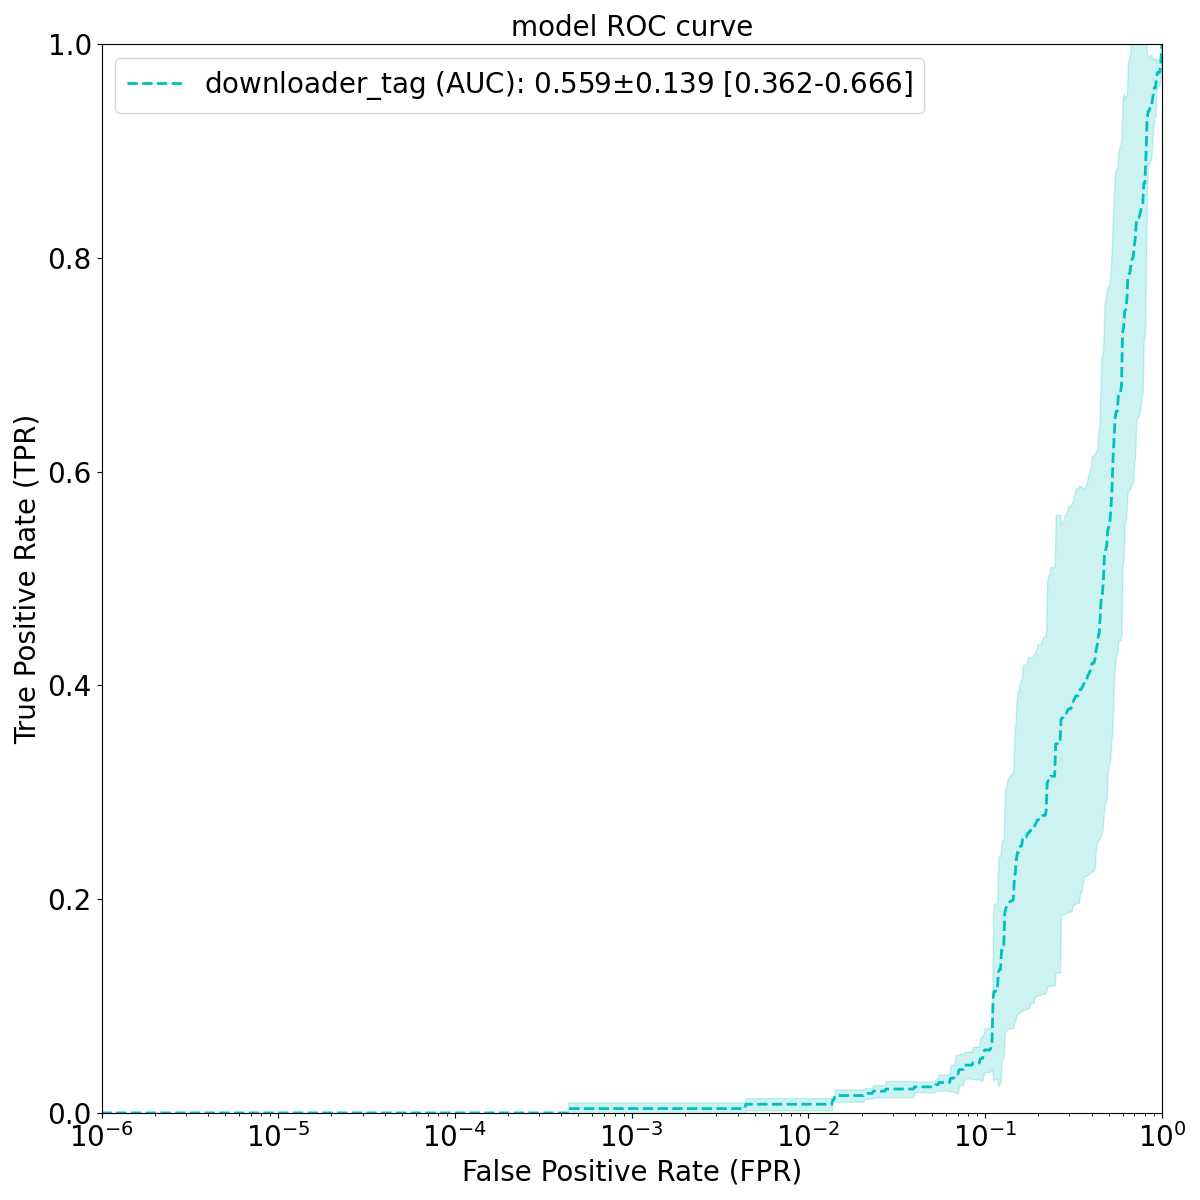
\includegraphics[width=0.6\textwidth]{./results/downloader_tag_roc_aloha.png}
        \vspace*{-0.2cm}
        \caption{ROC curve and AUC statistics of \textBF{ALOHA} model for the \textbf{Downloader Tag}. The line represents the \textit{mean} TPR at a given FPR, while the shaded region represents the \textit{standard deviation}. Statistics were computed over \textBF{3} training runs, each with random parameter initialization.}
        \label{fig:downloaderTagRocAloha}
    \end{figure}
}

\newcommand{\downloaderTagRocJointEmbedding}{
    \begin{figure}[H]
        \vspace*{-0.5cm}
        \centering
        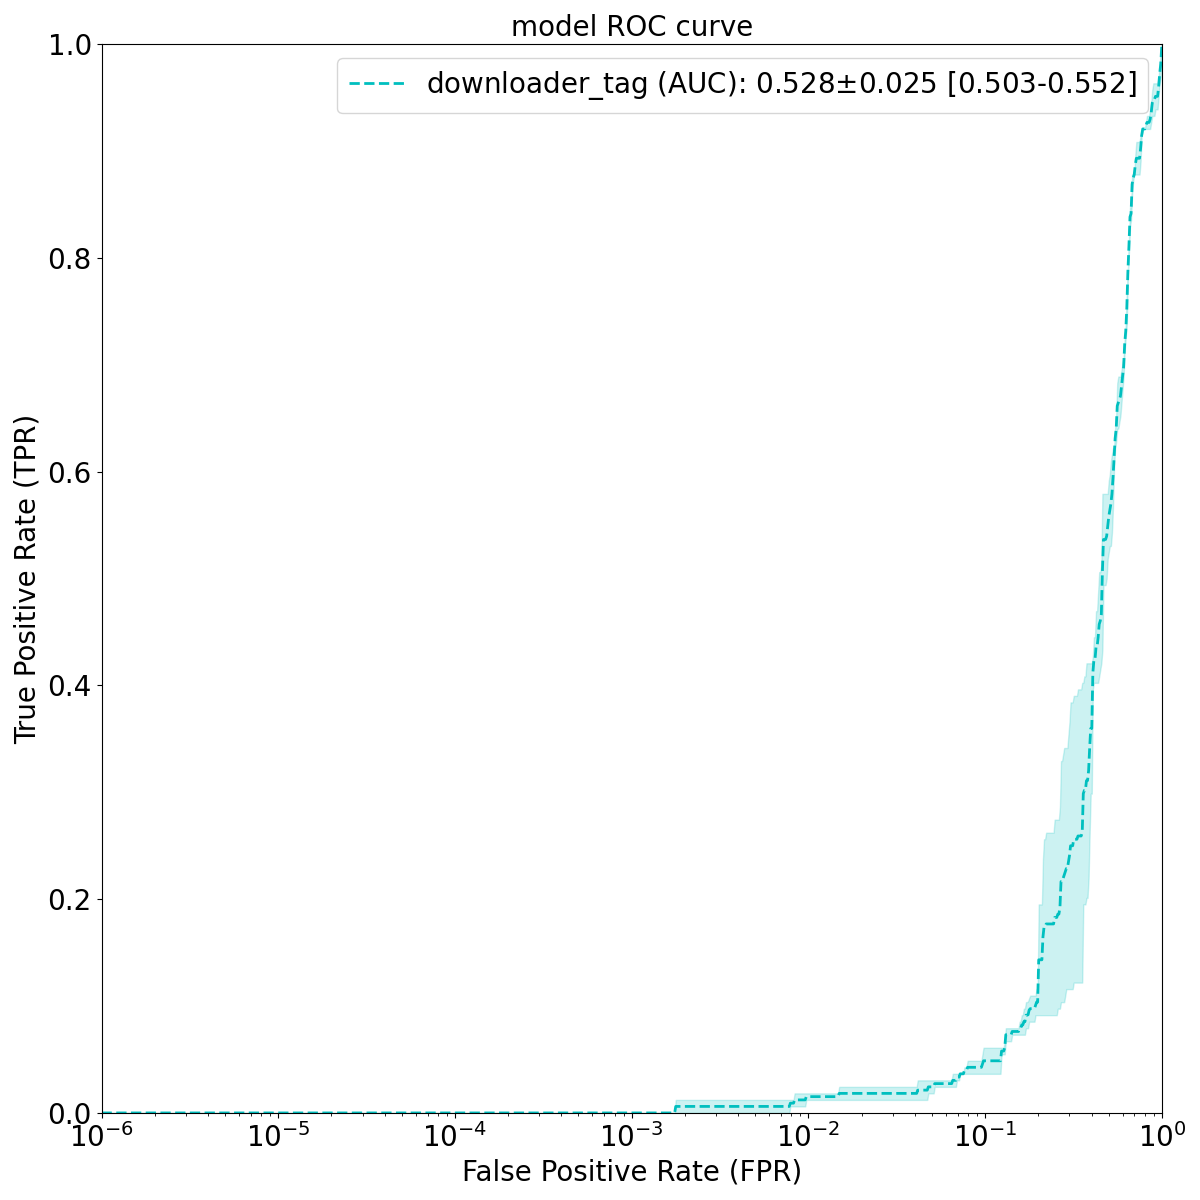
\includegraphics[width=0.6\textwidth]{./results/downloader_tag_roc_jointEmbedding.png}
        \vspace*{-0.2cm}
        \caption{ROC curve and AUC statistics of \textBF{Joint Embedding} model for the \textbf{Downloader Tag}. The line represents the \textit{mean} TPR at a given FPR, while the shaded region represents the \textit{standard deviation}. Statistics were computed over \textBF{3} training runs, each with random parameter initialization.}
        \label{fig:downloaderTagRocJointEmbedding}
    \end{figure}
}

\newcommand{\downloaderTagRocProposedMethod}{
    \begin{figure}[H]
        \vspace*{-0.5cm}
        \centering
        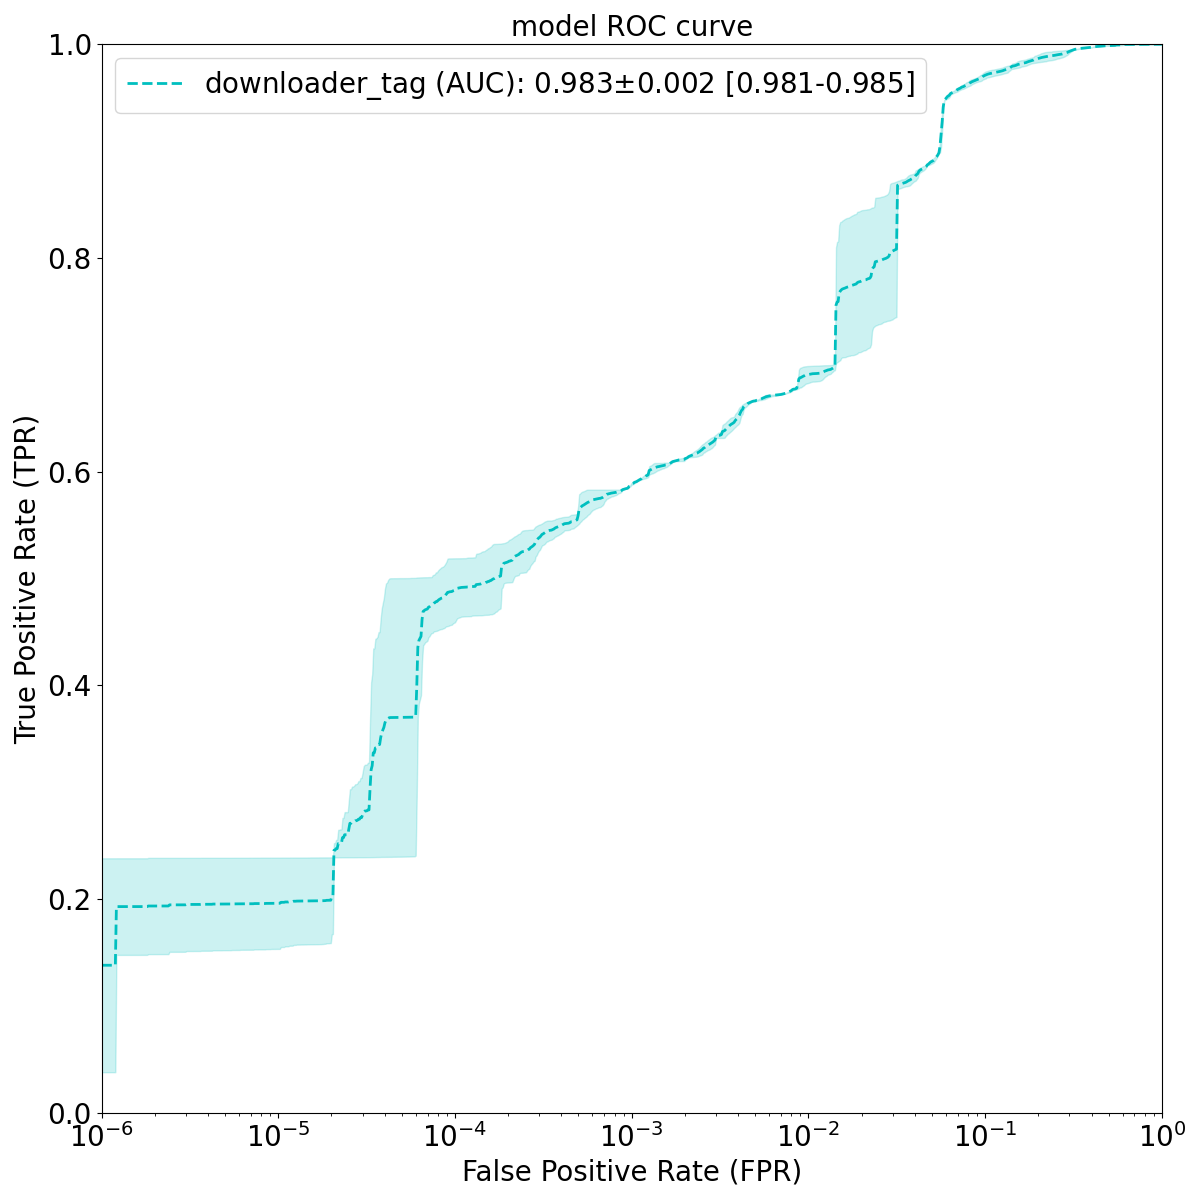
\includegraphics[width=0.6\textwidth]{./results/downloader_tag_roc_proposedModel.png}
        \vspace*{-0.2cm}
        \caption{ROC curve and AUC statistics of \textBF{Proposed Model} for the \textbf{Downloader Tag}. The line represents the \textit{mean} TPR at a given FPR, while the shaded region represents the \textit{standard deviation}. Statistics were computed over \textBF{3} training runs, each with random parameter initialization.}
        \label{fig:downloaderTagRocProposedModel}
    \end{figure}
}
